\documentclass[twoside,single]{lion-msc}

\title{{ \texttt{Picosecond Jitter of Picosecond Pulses}}}
\author{Andrea Maccarinelli}
\studentid{4535286}                           % check you student ID, LaTeX does not do this
\abstract{Motivations and guide to the general structure of the thesis among the different chapters ! Motivazioni : Quello di cui voglio parlare è inerente al contesto di sempre maggiore interesse al giorno d'oggi delle tecnologie sviluppate 			sulla base dei principi della quantum optics. A questo punto l'idea sarebbe quella di fare una breve picture storica, volta alla trasmissione al lettore del concetto secondo cui tutto 			questo ambito di ricerca sia estrememente recente e sebbene le prime avvisaglie sono state nei primi anni '50 con Glauber e HBT, il 			grosso arriva solo dagli anni 70-90.Il tutto conduce all'inizio del nuovo secolo quando con l'avvento degli SNSPD e la teorizzazione e creazione dei primi QD si è iniziato a parlare di "Modern Quantum Optics". La conclusione di questa parte di motivazioni io la farei andando ad introdurre il concetto del perfezionare la qualità della luce a singolo fotone che siamo in grado di produrre. Modern society is heading towards the massive use of quantum computing and quantum communication protocols for research purposes, as well as hopefully one day like a revolutionary mean of communication. All these technologies, far from being fully implemented with the state-of-the-art instruments find their functioning principles in the Quantum Optics theory. }     % limit your self to 1/2 page or 500 words
\supervisor{Dr. Wolfgang Loeffler}                         % Note that this should be a LION staff member!
\corrector{Dr. Evert van Nieuwenburg}                   % This could be a LION staff member or your external supervisor

\degree{Master of Science}                     % The default option is "Bachelor of Science", change if needed

%\major{Physics and Astronomy}                  % The default option is "Physics", change if needed
%\major{Physics and Mathematics}

% optional cover picture - should be jpg or pdf
% \coverpicture{\includegraphics[width=13cm]{thesisstyle.png}}

% Use this to make hyperlinks visible in the document.
% \hypersetup{colorlinks=true}

% ---------------------------------------------------------------- My defintions!
% \renewcommand{\vec}[1] {\ensuremath{ \overrightarrow{ #1 } }}
\renewcommand{\vec}[1] {\ensuremath{ \mathbf{ #1 } }}
% \bra \ket \braket and \proj
\newcommand{\bra}[1]{\ensuremath{\langle #1 \vert}}
\newcommand{\ket}[1]{\ensuremath{\vert #1 \rangle}}
\newcommand{\braket}[2]{\ensuremath{\langle #1 \vert #2 \rangle}}
\newcommand{\proj}[1]{\ensuremath{\vert #1 \rangle \langle #1 \vert}}

\newcommand{\kpar}{\ensuremath{k_\parallel}}
% ----------------------------------------------------------------

% \usepackage{tocloft}
% \renewcommand{\cftchapdotsep}{\cftdotsep}
\usepackage{comment}


% Redefine autoref names to be capitalized
\AtBeginDocument{%
  \renewcommand{\sectionautorefname}{Section}
  \renewcommand{\subsectionautorefname}{Subsection}
  \renewcommand{\chapterautorefname}{Chapter}
  \renewcommand{\figureautorefname}{Figure}
  \renewcommand{\tableautorefname}{Table}
  \renewcommand{\equationautorefname}{Equation}
}

% Optional: enable visible colored links (if hidelinks is unwanted)
% \hypersetup{
%   hidelinks=false,
%   colorlinks=true,
%   linkcolor=blue,
%   urlcolor=blue,
%   citecolor=blue
% }
\usepackage[table]{xcolor}
\usepackage{colortbl}
\usepackage{array}
\usepackage{caption}

\begin{document}

% roman numbering in the table of contents section
\pagenumbering{roman}

\maketitle

% Table of contents :  it is a good idea to include this into your thesis
\tableofcontents
\cleardoublepage

% The following list of figures and list of tables are optional. Remove the comments if needed
%\listoffigures
%\newpage

%\listoftables
%\newpage

% in the main part of the document use standard arabic numbers. Page counter resets to 1.
\pagenumbering{arabic}


%\maketitle

\chapter{Introduction}

\begin{comment}
    Motivations and guide to the general structure of the thesis among the different chapters !
\end{comment}

The current state-of-the-art quantum communications technologies base its functioning principles upon entangled states of single photons.
This is a completely new field, characterized by a very recent and still developing theoretical background. 
Although Quantum optics finds its roots in the 50s with the first discoveries brought by Glauber and Hanbury, Brown and Twiss, the key interest rose only in the decennia 70-90s.
Modern day quantum optics gained even more interest with the discovery of single photon light sources like quantum dots, as well as the introduction of ultra-fast single photon detectors : Technologies developed all after the advent of the new century. % that came into reality only at the beginning of the new century

In recent years the perspectives of a widely spread use of totally safe mean of communication based on quantum communication principles, is attracting like never the interest of public and private entities.
made possible by the
%The history of this research field, and its race towards a complete revolution of the means of communication currently drives the 
\chapter{Theory}

\section{Introduction to optical jitter}
\section{Temporal characteristics of optical pulses}
\section{Origins of jitter in experimental systems}
\section{Measuring and interpreting optical jitter}
\chapter{EOM ps pulses and correlations}
\label{Capitolo3}
In this chapter will be presented our study of an EOM based pulsed laser source to inspect the timing jitter.
\autoref{sec:Overview} will provide a comprehensive description of the experimental setup, to introduce a brief list of the jitter sources arising from the different components that will be located at \autoref{sec:Jitter Sources}.
We will then explain how the raw data are processed in \autoref{sec:DataAnalysis}, focusing in particular on \autoref{subsec:CentralPeakId} where the procedure behind the zero-delay peak recognition is explained.
Finally \autoref{EOMresults} presents the results we get from our analyses.


\section{Experimental setup overview}
\label{sec:Overview}
\begin{comment}

    These are the independently measured pulse lengths (FWHM), as function of the electrical bias imposed in the pulse compressor card.
    pulse_length[pulser_delay] = {-75.0: 22.332656690670724, -70.0: 33.28737362600773, -65.0: 34.562790842683, -60.0: 37.234513127783835, -55.0: 39.60844036795933, -50.0: 41.46464279128635, -45.0: 44.179758740180006, -40.0: 47.14183222708421, -35.0: 49.84367579880712, -30.0: 52.69148088494188, -25.0: 55.55398638871779, -20.0: 58.29172752901992, -15.0: 61.56981413564056, -10.0: 65.10148899764842, -5.0: 68.5853235124889, 0.0: 72.17479431215992, 5.0: 75.30042828585228, 10.0: 78.37782629223706, 15.0: 81.35991580449851}

    Queste misure sono state prese con un solo EOM, anche se l'autore riferisce che per pulse delays maggiori di -60 la lunghezza riportata qui corrisponde a quella che si osserverebbe nella configurazione con due EOM che invece utilizzo io nella mia tesi.
\end{comment}


For this first experimental chapter of this thesis we used a pulsed laser source originated by the use of electro-optic modulators (EOMs) on a starting CW laser source.
In \autoref{EOM_Setup_BIG} a zoomed out sketch of the experimental setup can be found. The image shows how the CW laser is coupled into a polarization-maintaining single-mode fiber (PM-SMF), and then electro-optically modulated by electronic signals shaped by a high-speed electronic circuit. All these components belong to the Orange shaded area of the picture.
On behalf of the electrical bias imposed in the PC interface, this part of the setup is responsible for the creation and the modulation of the optical pulses, according to an electronic delay imposed via PC.

The resulting pulsed laser source is then attenuated in intensity using a fiber splitter and then transferred with another fiber to the HBT setup, represented in \autoref{EOM_Setup_BIG} with a green colored area.
In this part of the setup the beam is equally divided with a fiber directional coupler, and then plugged into the second and third detectors of our SNSPD. As introduced in \autoref{sec:Def-Techniques}, the raw data, consisting of time-tagged detection events recorded by the ID1000 time tagger, will later be used to compute coincidences. These two final instruments consist in a "ID281" SNSPD together with a "ID1000" time tagger, both manifactured by ID Quantique SA.
For the specifications of the other components we remind to the article of the original designer of this setup, Mio Poortvliet \cite{MioArticle}.

\begin{figure}[hbtp]
\centering
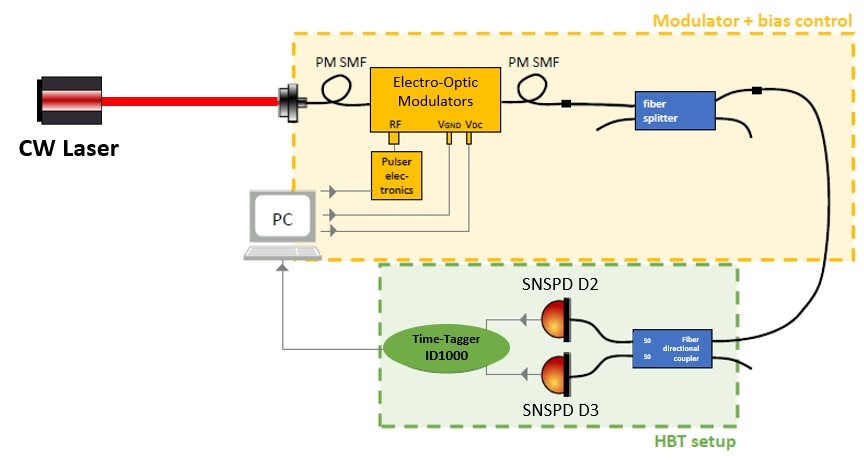
\includegraphics[width=1\textwidth]{EOMsetupBIG.jpg}
\caption{Schematic representation of the EOM based experimental setup}
\label{EOM_Setup_BIG}
\end{figure}
It is worth noting that in \autoref{EOM_Setup_BIG} the electro-optic modulation and the electronics that drives it, are only minimally shown. \autoref{EOM_PulseGen} provides a more detailed insight on what is actually driving the pulse generation.
The first three blocks from the top of the image represent the high speed electronics that generates the driving signal of the two EOMs.
At the very first stage, a field-programmable gate array (FPGA) generates a trigger signal in the form of a pulse pattern, that is passed to the pulse generator card. This system cam be operated in two regimes. For this project we specifically use the fast pulse generator, with a resolution of 1 ns and a configurable repetition rate ranging from 8 MHz to 500 MHz.
In our case the FPGA generates 1ns long pulses at the desired repetition rate of around 65MHz, corresponding to a repetition period of 15.2 ns.  
At this point, the signal is split and sent to two programmable delay lines with a resolution of 5 ps; a delay is applied to only one of the copies.
These two refined signals are combined with a 14-Gbps AND gate to obtain the customized pulse pattern whose width is adjustable based on the user-defined bias values for the programmable delay lines that we mentioned earlier.
Subsequently, the outputs of the pulse compressor board are the two pulse patterns resulting from a XOR port fed with the previous signal and a constant reference signal.

These two outputs, upon previous amplification, are then connected to the RF electrodes of the two cascaded EOMs, whose configuration is depicted in the lower part of \autoref{EOM_PulseGen}.  

\begin{figure}[hbtp]
\centering
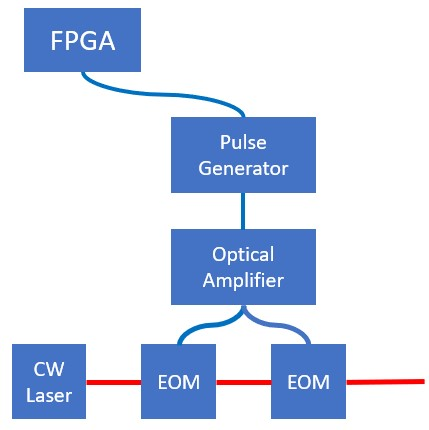
\includegraphics[width=0.4\textwidth]{EOM_Pulse_Sketch.jpg}
\caption{Schematic representation of the experimental tools involved into the pulse generation}
\label{EOM_PulseGen}
\end{figure}

\section{Relevant jitter in this experiment}
\label{sec:Jitter Sources}
After presenting the experimental architecture, this section examines the dominant sources of timing jitter introduced by the various components described above.
The pulser electronics encloses the first and main sources of timing jitter.
Referencing \autoref{EOM_PulseGen}, we identify within the FPGA, the first source of jitter, strictly followed by the effect of the several input discriminators implied in the architecture of the pulse generator card\cite{MioArticle}. The final purity affecting source, for this part comes from the ps-signal amplifier.
We assume that the electro-optic modulation of the CW laser is jitter-free, and that group velocity dispersion (GVD) only causes a slight temporal broadening of the pulses, without introducing significant distortions that could lead to timing jitter.
Focusing once again on \autoref{EOM_Setup_BIG}, it is worth noting that the time-tagged detection events collected from the ID1000 are also affected by other jitter contributions, at this point strictly related to the detection and processing routines in the two final instruments involved.
The single photon detector carries an intrinsic system-jitter contribution, and this is still an open research topic in the field of the SNSPDs \cite{SNSPD_Jit_1, SNSPD_Jit_2}.
Subsequently, as previously introduced, the electrical signals generated by the SNSPD are transferred to the time tagger. The ID1000 performs click identification based on a defined detection threshold; an improper choice of this threshold can cause delayed detections, introducing a deterministic source of jitter.
To the best of our knowledge, there may also be a contribution to timing jitter arising from internal clock drifts within the ID1000.

It is worth mentioning that, since we extensively use cables, we cannot exclude the possibility that electromagnetic noise—such as crosstalk—could introduce deterministic timing jitter at multiple points in the setup.

\section{Data analysis}
\label{sec:DataAnalysis}
To understand some of the passages that distinguish the data analysis it is necessary to mention before the experimental procedure that lead us to achieve the raw data that we used for our analysis.
The data acquisition is divided into two different moments : Pulse refining and data acquisition.
The first part is focused in defining the shape of the optical pulses. Setting initially the delay to the pulse compressor board, and optimizing for the transmission of the two EOMs leads to the production of our optical pulses.

Subsequently, via software we set up the software to do two separate TCSPC on the two detectors using as reference to start the clock the same pulse pattern with period 15.2 ns that also drives the EOM transmission.
The Time tagger measures the amount of relative time between the reference signal and the detection.
Every measurement lasted 15 seconds, and each one is related to a different electrical delay value.

In total, 5 measurements have been saved, corresponding to these delays $d \in \{-10,-25, -35, -50, -60\}$ [ps]

The resulting raw data, corresponding to a single 15-second measurement, consists of two binary files, each representing a stream of time-tagged detection events from one of the two detectors.
After appropriate reshaping, each file appears as a two-column array: the first column ($t_{\text{rel}}$) indicates the time difference, in picoseconds, between the detection event and the preceding reference signal, while the second column ($T_{\text{clk}}$) provides the index of the reference event to which the detection is associated.
%Qui inizio a spiegare come abbiamo letto questi dati !!!
% Finally, every  and is the result \autoref{eq:Timestamps}.
To correlate each detection event we then need to convert such binary files into actual streams of detections.
For this reason, since the indeces of the reference events are expressed in units of the FPGA, by multiplying such values for 15200 ps, the repetition period of the laser, we will compute macroscopically the time of the detection event.
The microscopical difference of time between the detection and the reference, provides finally the missing piece to retrieve the absolute time of the click.
The resulting stream of detections is then composed by values computed as shown in \autoref{eq:Timestamps}.

\begin{equation}
    t_{\text{abs}} = i \cdot T_{\text{clk}} + t_{\text{rel}}
\label{eq:Timestamps}
\end{equation}

\begin{comment}
These two streams of detections are then computed to retrieve the histogram of the coincidence counts. This procedure has its foundations on the assumption of an initial detection, and following to that the detection within a maximum shift distance in time are identified. The resulting coincidences are then binned onto an histogram, assuming a certain binsize. By these means there are two main variables, that determine the quality of the data collected : $\Delta \tau _{max}$ as well as the width $\delta \tau$ of the bins.

\begin{figure}[hbtp]
\centering
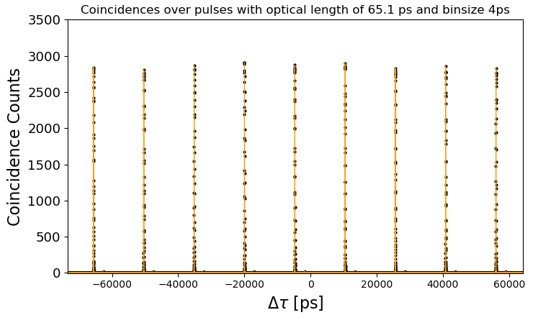
\includegraphics[width=1\textwidth]{CoincidenceExample.jpg}
\caption{Plot showing coincidence counts versus time, expressed in picoseconds. Image related to a measurement with a bias of -10 ps, correspoding to an independently measured duration of the pulse of 65.1 ps}
\label{CoincidenceCounts}
\end{figure}

\end{comment}


\subsection{Data processing pipeline}
\label{subsec:Pipeline}



These two streams of detections are then computed to retrieve the histogram of the coincidence counts. This procedure has its foundations on the assumption of an initial detection, and following to that the detection within a maximum shift distance in time are identified. The resulting coincidences are then binned onto an histogram, assuming a certain binsize. By these means there are two main variables, that determine the quality of the data collected : $\Delta \tau _{max}$ as well as the width $\delta \tau$ of the bins.
Since these are count-based histograms, the error related to each one of these coincidences corresponds to the square root of the number of counts detected.
\autoref{CoincidenceCounts} shows how such coincidences are displayed over the shift time of arrival : the periodic nature of such peaks reflects the periodicity of the optical pulses.

\begin{figure}[hbtp]
\centering
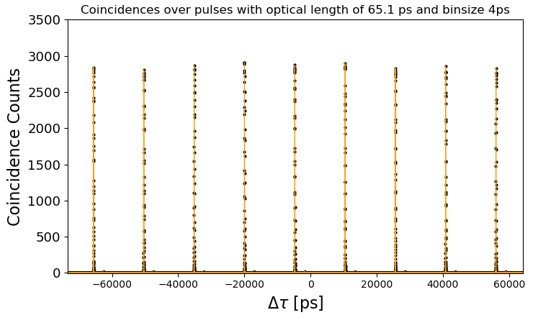
\includegraphics[width=0.75\textwidth]{CoincidenceExample.jpg}
\caption{Plot showing coincidence counts versus time, expressed in picoseconds. Image related to a measurement with a bias of -10 ps, correspoding to an independently measured duration of the pulse of 65.1 ps}
\label{CoincidenceCounts}
\end{figure}



At this precise point, we implement the procedure of normalization explained in  \autoref{subs:HBT}, more specifically using \autoref{Martinez_g2}.

The key point of this part is to analyse the $g^2 (\tau)$ peaks, automatizing the simultaneous fit of every one of them.
Left and right boundaries of the fitting intervals related to each peak were reconstructed starting from an initial pair, observed graphically.
All the others were retrieved adding or subtracting multiples of the repetition period of the pulsed laser source, that we remember being 15.2 ns.
\autoref{FittingIMG} (a) shows how using dashed and non dashed red lines, the fitting intervals are identified among the x-axis.

The gaussian function used to fit the $g^2 (\tau)$ peaks is \autoref{GaussianFit}, where the relation between the FWHM and the sigma is portrayed in \autoref{eqFWHM}. 
\begin{equation}
y(x) = A \, \exp\!\left( -\frac{1}{2} \left( \frac{x - d}{\sigma} \right)^{2} \right) + b
\label{GaussianFit}
\end{equation}

\begin{equation}
\sigma = \frac{\mathrm{FWHM}}{2 \sqrt{2 \ln 2}}
\label{eqFWHM}
\end{equation}

\autoref{FittingIMG} (b) shows one of the resulting gaussian fits.
The resulting parameters resulting from each one of these fits will then be saved into an array of pandas dataframes, ready for any further computation.
\begin{figure}[hbtp]
\centering
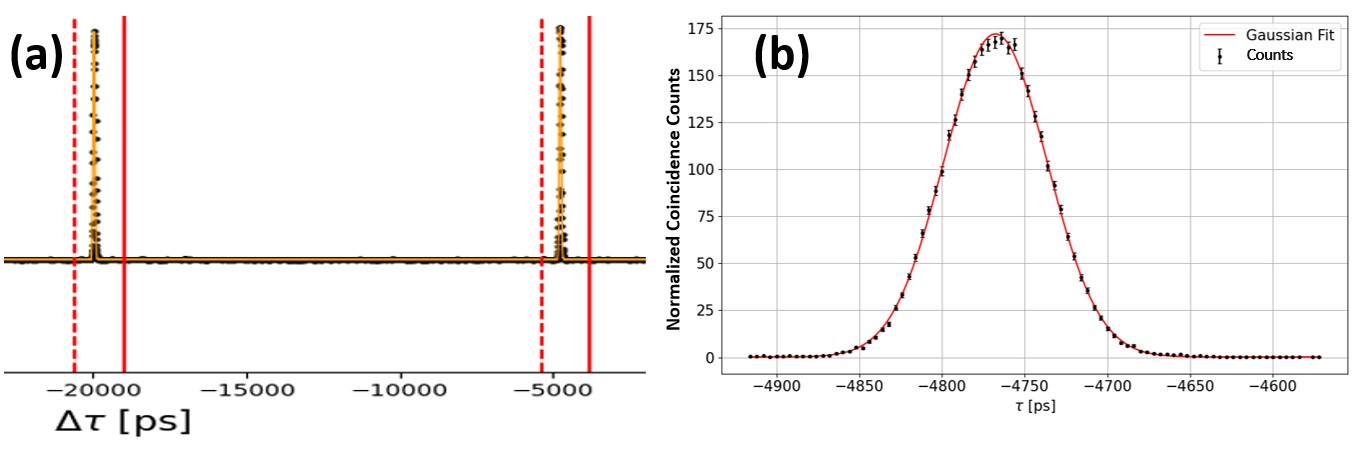
\includegraphics[width=1\textwidth]{NCountsFitting.jpg}
\caption{(a) Visual representation of the fitting intervals related to two different peaks. The red-dashed line represents the left boundary while the steady red one the right one. (b) Example of the gaussian fit obtained for one peak of the normalized counts plot.}
\label{FittingIMG}
\end{figure}

%\newpage
\subsection{Central peak identification}
\label{subsec:CentralPeakId}
At the current stage, the peaks are not displayed over the correct x axis, this is because we just limited our analysis to the fit of the $g^2 (\tau)$ peaks. We still have to identify the Zero-time delay peak, that will be later also referenced as the  $\Delta \tau = 0$ peak.

The main intuition towards the identification of this peculiar peak came from \autoref{FWHMvsTauSingle}.
In this image are displayed the FWHMs of all the $g^2 (\tau)$ peaks versus the position in the x axis.
Despite the presence of a vast number of peaks having on average the same width, there are two clear candidates that exhibit a significant less value.
Among these two candidates we identify as the Zero-time delay peak the one with the least intense width.
Subsequently, we shifted the x axis for the value of this peak, in order to retrieve the desired scenario where for zero time delay there is the actual zero time delay peak.

The key reason behind this choice lies in the intrinsic meaning of this central peak, resulting directly from the coincidence counts at zero periods of distance. This motivates what we see in the plot where only two points show lower FWHM values, while the others do show an higher average value.
Technically we would expect only one clear minima, not two, but we think that the second one arises as a consequence of the use of two cascaded EOMs.


\begin{comment}
Qui ci sarebbe da dire che io nel codice a questo punto faccio un ultimo giro di fit sugli array finalmente corretti per la coordinata temporale del picco centrale.
\end{comment}


%\autoref{FWHMvsTauSingle}
\begin{figure}[hbtp]
\centering
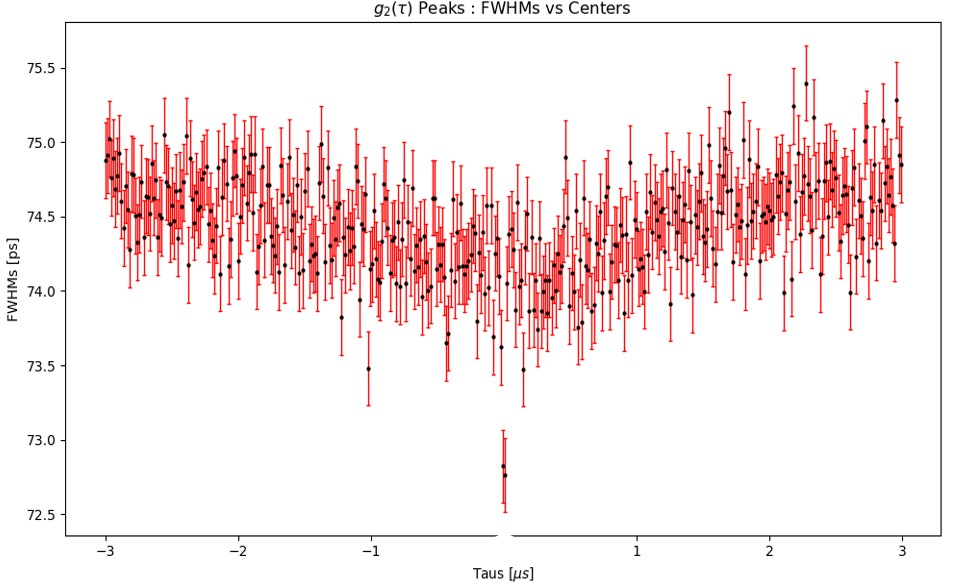
\includegraphics[width=1\textwidth]{FWHMvsTAU_Single.jpg}
\caption{Plot representing the FWHMs over the time shift coordinates $\tau$ of every peak fitted for one single measurement file. In the lower part of the center of the image can be notices two clear minima points.}
\label{FWHMvsTauSingle}
\end{figure}

%Aggiungere un paio di frasi per motivare la scelta in questo modo.
%Sottolinea che i picchi contengono informazioni sulla auto correlazione a diverse scale di distanza.
%Appare più che plausibile che il picco a zero delay mostri una minore larghezza, in quanto non risente già 
%del jitter della FPGA che inizia inevitabilmente a comparire poi...

\section{Results and Discussion}
\label{EOMresults}
Let us now discuss the results of this first part of the project by showing a selection of plots containing datas from 5 different measurements together.
Of these different measurements, obtained by varying the bias value on the pulse compressor board, we do have an independent measure of the resulting optical pulses. A proper legend has been added to each one of the plots to give notice to the duration values of these optical pulses.

\autoref{FWHMvsTauGeneral} presents a broader version of the plot described when we first introduced the zero time delay identification, this time with 5 different measurements. For each measurement minima points can be seen. 
Also, we notice how the average value of the FWHM per single population decreases with the decrease of the optical length of the pulses. It is worth mentioning, in this sense that the difference between the average FWHM value that we see in the main plot and the width of the pulse is caused primarily by the jitter of the system.
The contribution of the jitter increases with shorter pulses : The origin of this effect is still unclear.

\begin{figure}[hbtp]
\centering
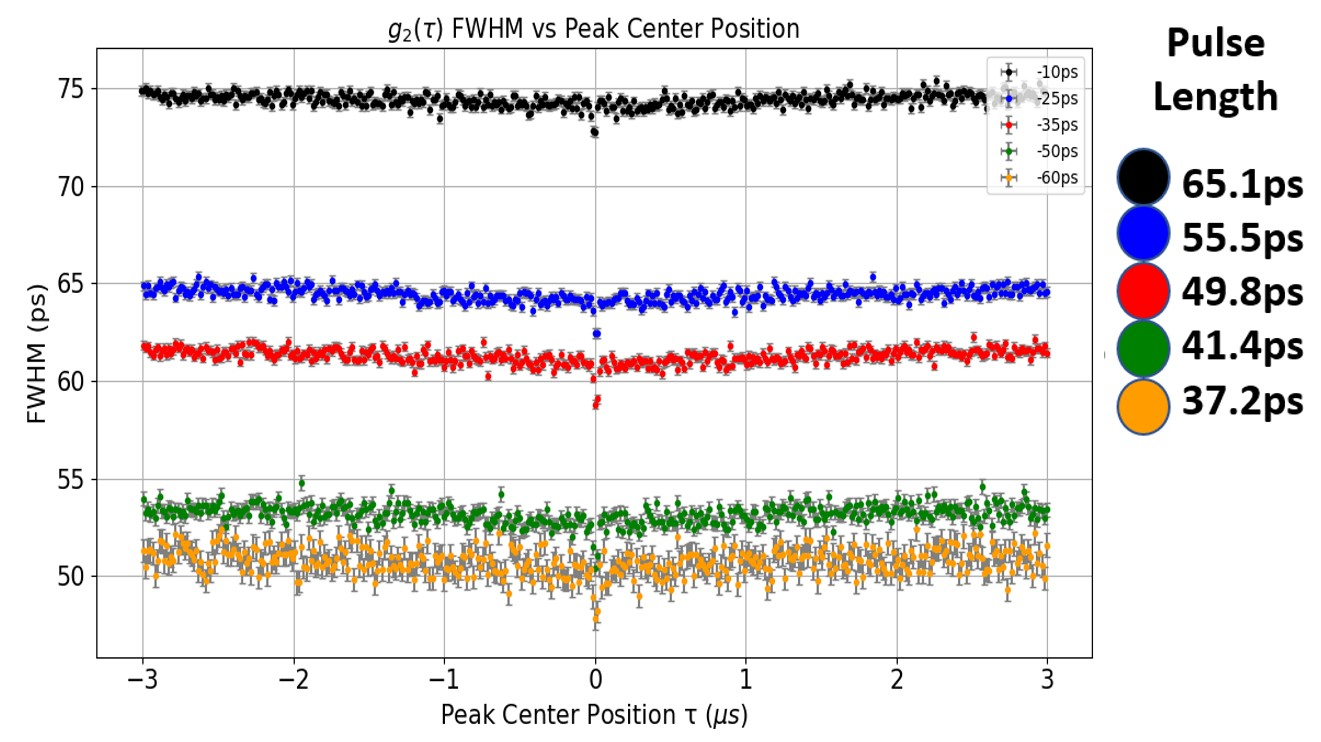
\includegraphics[width=1\textwidth]{FWHMvsTAU_ALL_Version2.jpg}
\caption{Measured FWHMs over the shift $\tau$ from the zero-delay peak. The colors represent the 5 different measurements obtained varying the bias value on the pulse compressor board. An independent measure of the corresponding duration of the pulses for each color is located in the legend on the right part of the image. }
\label{FWHMvsTauGeneral}
\end{figure}

Subsequently, we focused on the analysis of the variations of the widths of the peaks. According to the reasons explained previously behind the identification of the zero delay peak, we chose as reference for this study of the variations the zero delay peak.
On this behalf we displayed in \autoref{DeltaFWHMvsPERIOD_General} on the y axis these variations defined according to \autoref{DELTAEXP}

\begin{equation}
\Delta FWHM (N) = FWHM(N) - FWHM(0) 
\label{DELTAEXP}
\end{equation}
In particular with the letter "N", we refer to the number of periods of distance from the central peak. With this formulation the width variation related to the peak located at negative 15 periods from the central reference is displayed at  $x = -15$ on the x-axis.

Furthermore, \autoref{DeltaFWHMvsPERIOD_ZOOM} is a zoomed in version of the bigger \autoref{DeltaFWHMvsPERIOD_General}, that keeps the color scheme adopted for this section.

About these two images, depicting the variations of the FWHMs over the period number, some observations can be made :

\begin{itemize}
\item $\Delta FWHM(N)$ is smallest for $n \pm 1$
\item Outside $n \pm 1$ the variations gets larger and increase steadily over an interval of 10s of periods
\item For measurements related to longer pulses the variation appears to be smaller		
\end{itemize}


%Aggiungere qui le conclusioni che trovi nel documento condiviso

\begin{figure}[hbtp]
\centering
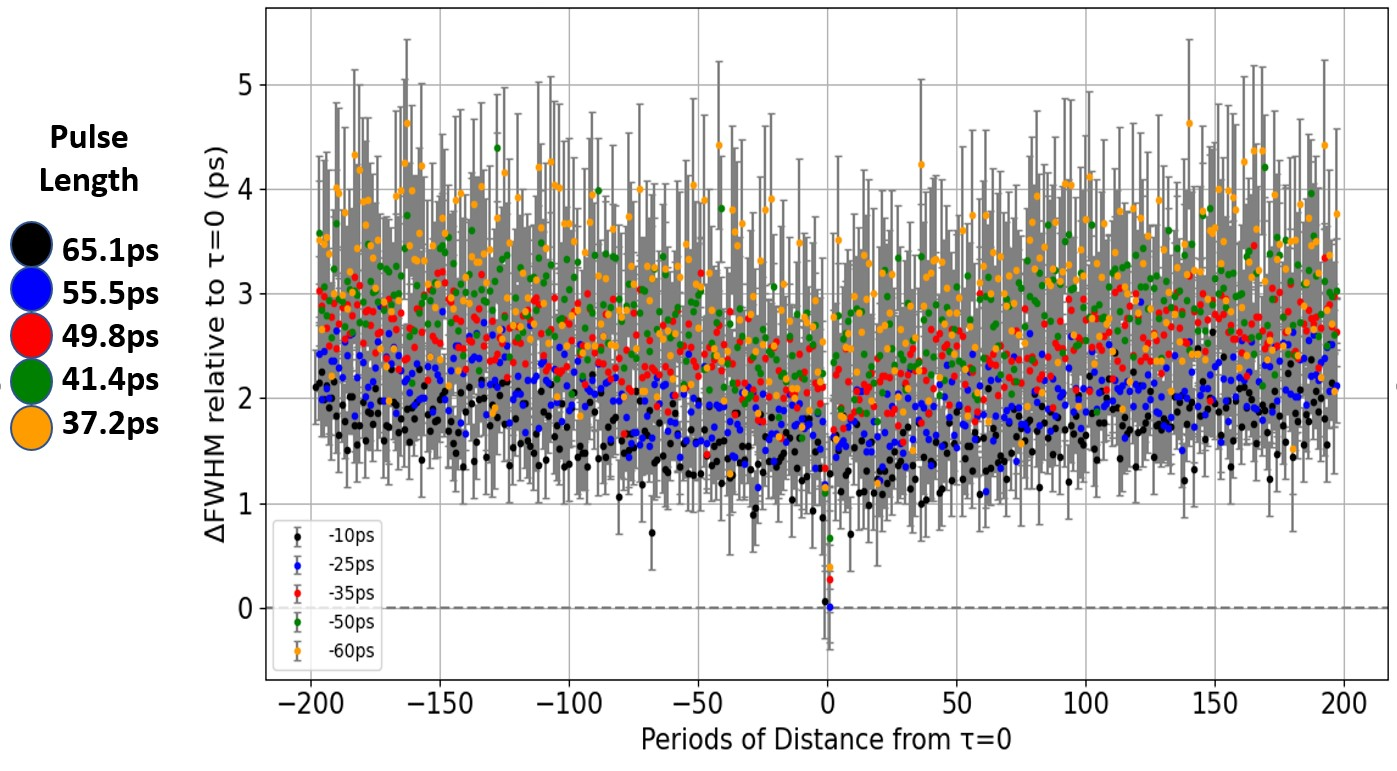
\includegraphics[width=1\textwidth]{DeltaFWHMvsPeriods.jpg}
\caption{Measured FWHM variations computed with respect of the central peak, chose as reference for its intrinsic properties. The results are plotted at the specific coordinate on the x-axis related to the peak to which the variation is related, according to \autoref{DELTAEXP}. On the Left side there is a legend that relates the colors of the points in the plot with an independent measure of the pulses being for each experiment.}
\label{DeltaFWHMvsPERIOD_General}
\end{figure}

\begin{figure}[hbtp]
\centering
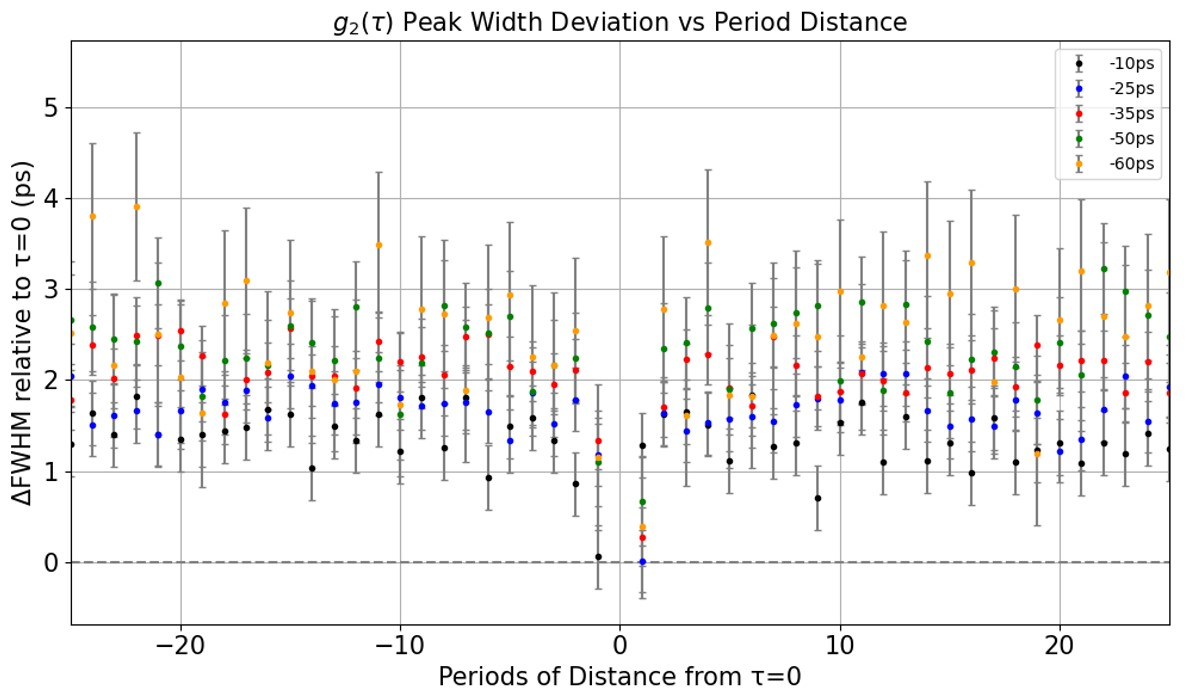
\includegraphics[width=1\textwidth]{DeltaFWHMvsPeriods_ZOOM.jpg}
\caption{Zoomed in version of \autoref{DeltaFWHMvsPERIOD_General}, limited over a range of $\pm 25$ periods from the central zero-delay peak. The difference between the first two points from the center and the others is here more evident. There is not value displayed in the origin of the axis, for each one of the measurenents. We chose to not display it with purpose, since according to \autoref{DELTAEXP} this would result in a constant null value regardless of the dataset.}
\label{DeltaFWHMvsPERIOD_ZOOM}
\end{figure}

\chapter{Optimizing SNSPD HBT and TCSPC measurement of a fs laser source}


\section{Motivations and experimental setup overview}
\begin{figure}[hbtp]
\centering
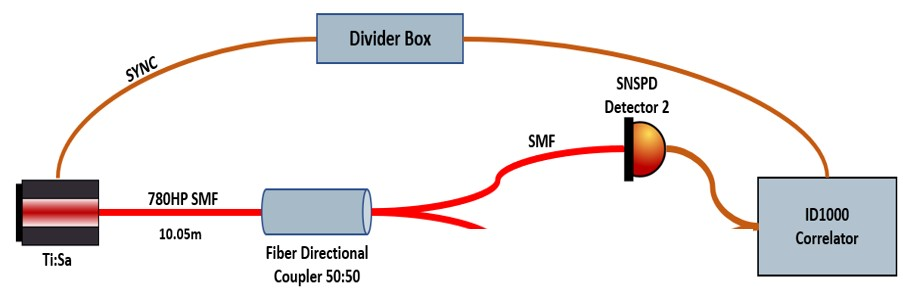
\includegraphics[width=1\textwidth]{TiSa_Setup.jpg}
\caption{Ciaone}
\label{TisaSetup}
\end{figure}



\section{Unwanted Side Peaks in HBT and TCSPC measurements}

\begin{figure}[hbtp]
\centering
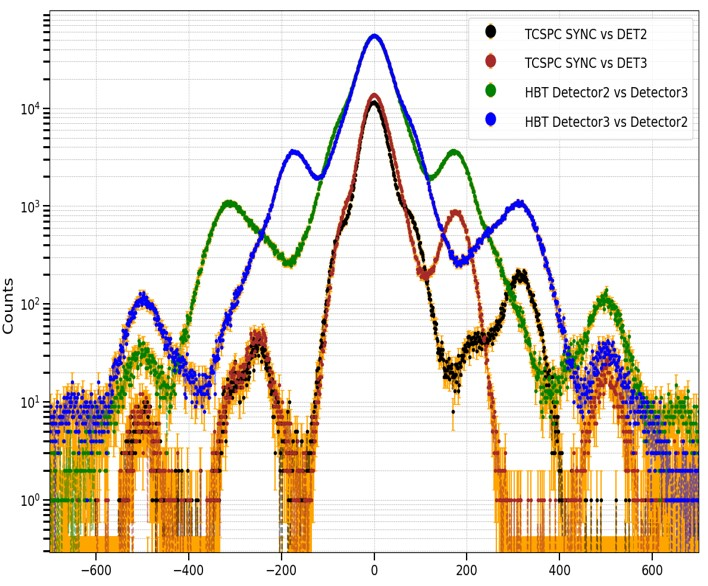
\includegraphics[width=1\textwidth]{Khaos.jpg}
\caption{Ciaone}
\label{Khaos}
\end{figure}
\section{Partly retrieving side peaks in HBT from coordinates of TCSPC peaks}

\begin{figure}[hbtp]
\centering
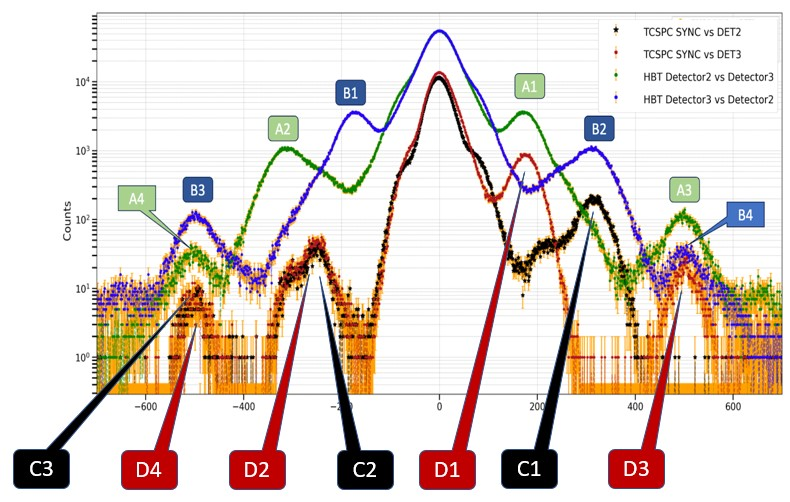
\includegraphics[width=1\textwidth]{Khaos_Labeled.jpg}
\caption{Ciaone}
\label{Khaos_labeled}
\end{figure}
\section{Measurements with improved detection thresholds}
\subsection{Driving idea}
\subsection{Discussion of the new measurements}
\subsection{Estimation of the width of the Detector response function}
\chapter{Conclusions and outlook}





\bibliographystyle{plain}
\bibliography{bibliography}
\end{document}

